\documentclass[tikz,border=12pt]{standalone}
\usepackage[T1]{fontenc}
\usepackage{mathpazo}
\usepackage{amsmath,amssymb}
\usetikzlibrary{arrows.meta, calc}

\definecolor{stblue}{HTML}{7B97AD}
\definecolor{rwgold}{HTML}{B8995E}
\definecolor{sage}{HTML}{7A9A7E}
\definecolor{dkbrown}{HTML}{3D3530}
\definecolor{wmgray}{HTML}{7B7067}
\definecolor{cream}{HTML}{F9F6F0}
\definecolor{border}{HTML}{D4C9B8}
\definecolor{terracotta}{HTML}{C47A6A}
\definecolor{lavender}{HTML}{907EA0}

\begin{document}
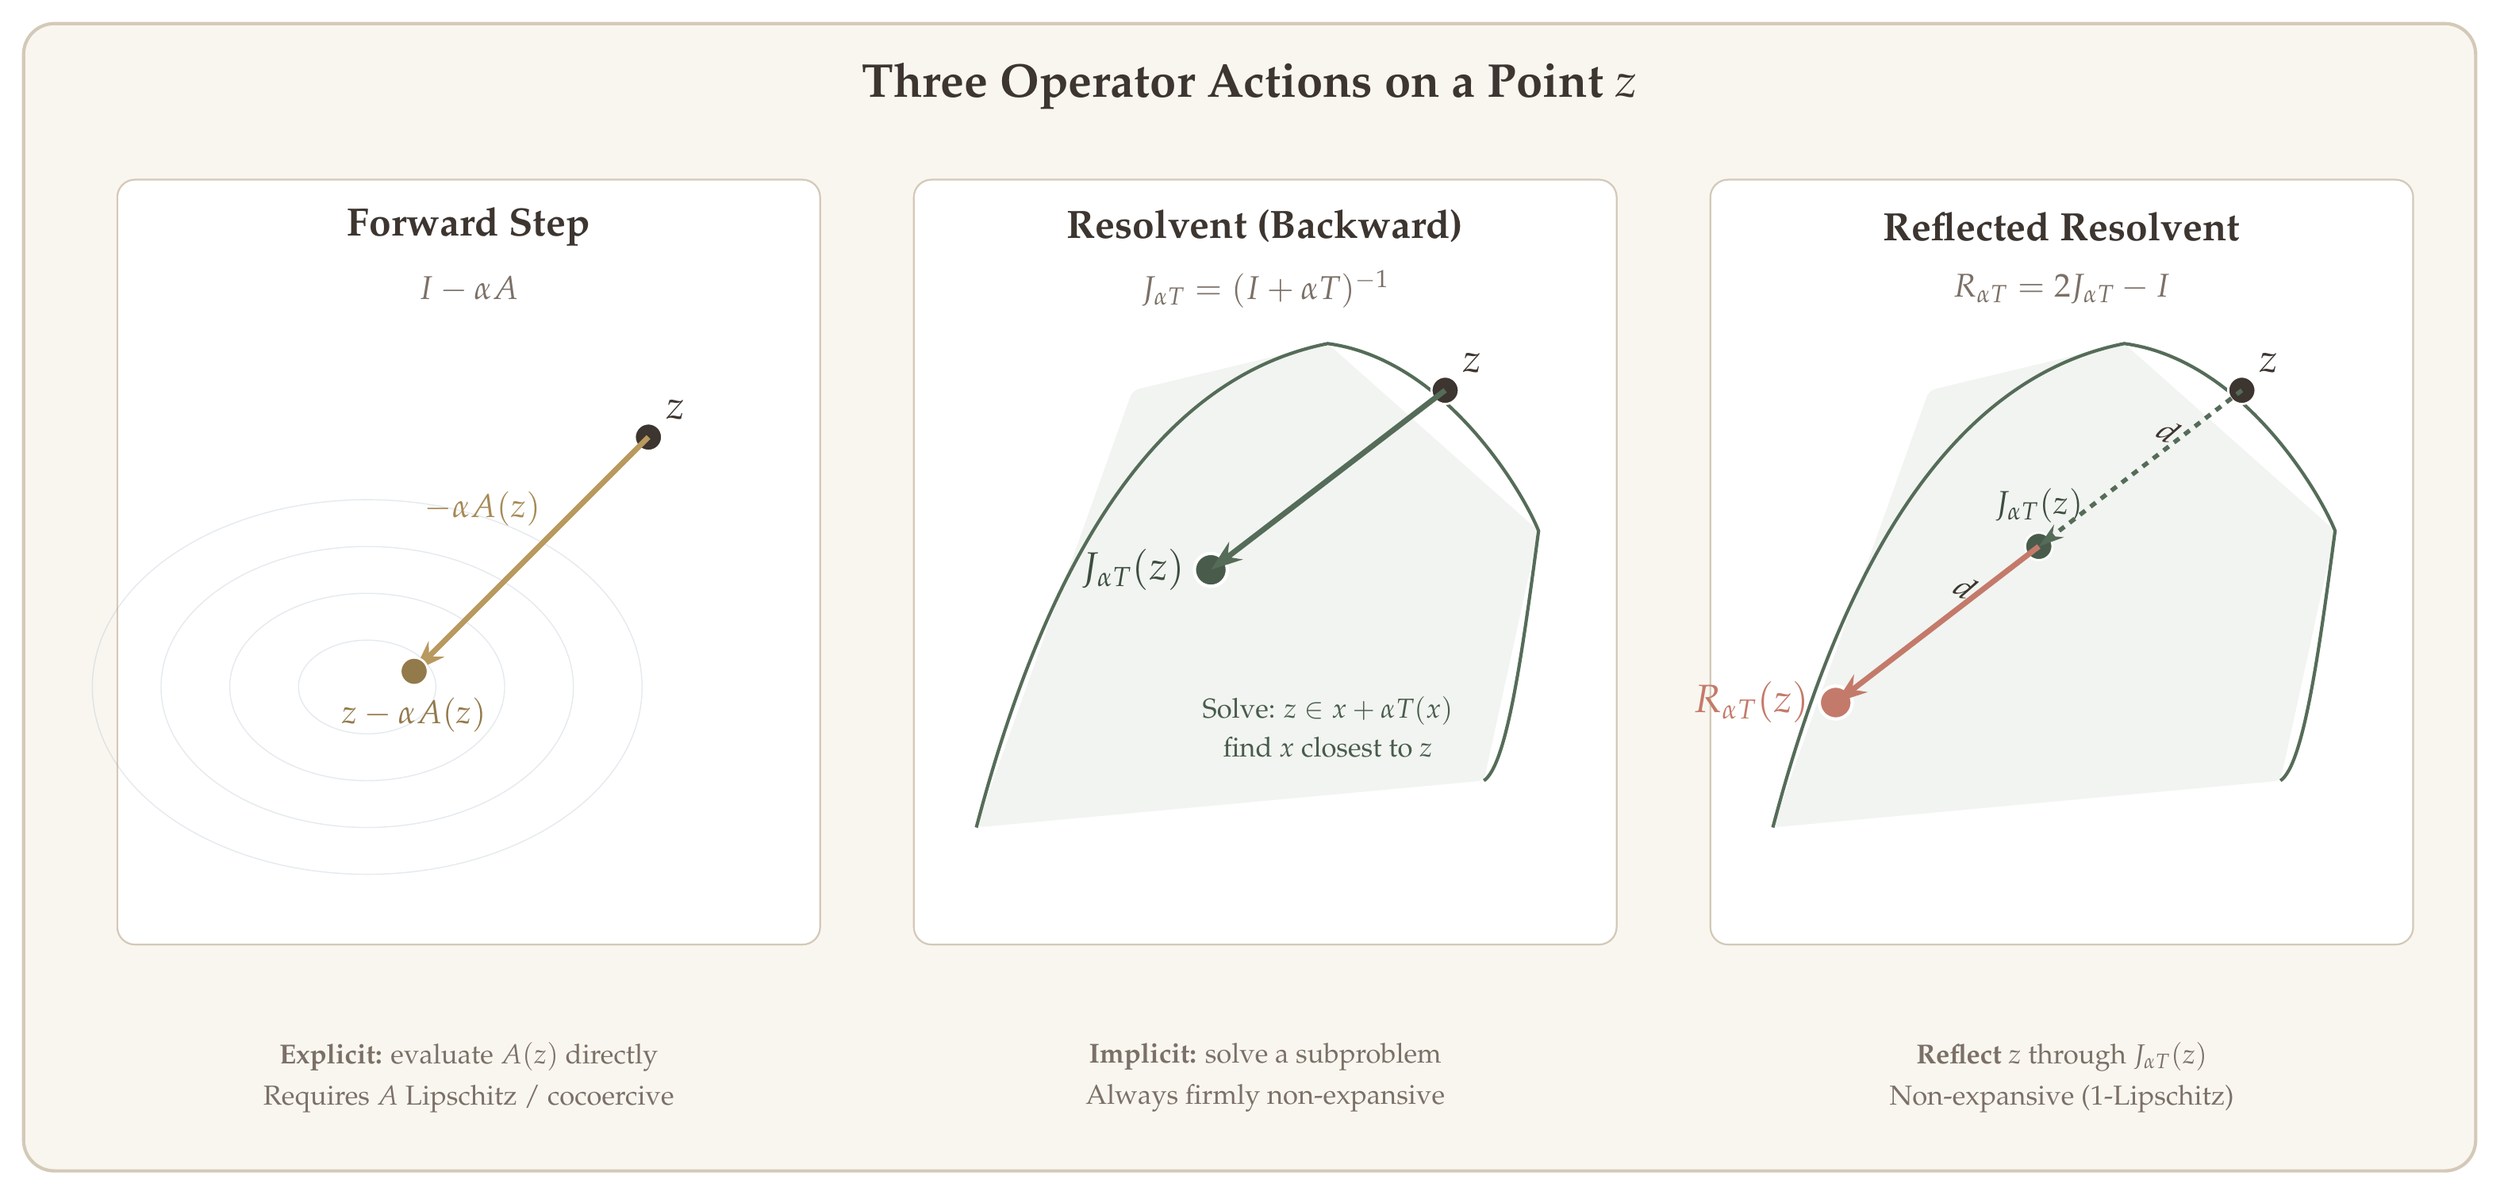
\begin{tikzpicture}[>={Stealth[length=4mm, width=3mm]}, scale=1.25, every node/.style={scale=1.25}]

% ============================================================
% Background
% ============================================================
\fill[cream, rounded corners=14pt] (-1.2,-3.2) rectangle (30.2,11.5);
\draw[border, line width=1.5pt, rounded corners=14pt] (-1.2,-3.2) rectangle (30.2,11.5);

% Title
\node[text=dkbrown, font=\LARGE\bfseries] at (14.5,10.7)
  {Three Operator Actions on a Point $z$};

% ============================================================
% Panel 1: Forward operator  I - alpha A
% ============================================================
\fill[white, rounded corners=8pt] (0.0,-0.3) rectangle (9.0,9.5);
\draw[border, line width=0.8pt, rounded corners=8pt] (0.0,-0.3) rectangle (9.0,9.5);
\node[text=dkbrown, font=\Large\bfseries] at (4.5,8.9) {Forward Step};
\node[text=wmgray, font=\large] at (4.5,8.1) {$I - \alpha A$};

% Contour lines (suggest landscape of f)
\foreach \r in {0.8, 1.6, 2.4, 3.2} {
  \draw[stblue, line width=0.5pt, opacity=0.2]
    (3.2,3.0) ellipse ({\r*1.1} and {\r*0.75});
}

% Point z
\coordinate (z1) at (6.8,6.2);
\fill[dkbrown] (z1) circle (5pt);
\draw[white, line width=1pt] (z1) circle (5pt);
\node[text=dkbrown, font=\Large\bfseries, above right=3pt] at (z1) {$z$};

% Gradient arrow from z
\coordinate (fwd1) at (3.8,3.2);
\draw[rwgold, line width=2.5pt, -{Stealth[length=5mm, width=3.5mm]}]
  (z1) -- (fwd1);
\node[text=rwgold!90!black, font=\large\bfseries, above left=0pt]
  at ($(z1)!0.42!(fwd1)$) {$-\alpha A(z)$};

% Result point
\fill[rwgold!80!black] (fwd1) circle (5pt);
\draw[white, line width=1pt] (fwd1) circle (5pt);
\node[text=rwgold!80!black, font=\large\bfseries, below=6pt] at (fwd1)
  {$z - \alpha A(z)$};

% Annotation
\node[text=wmgray, font=\normalsize, align=center] at (4.5,-2.0)
  {\textbf{Explicit:} evaluate $A(z)$ directly\\[3pt]
   Requires $A$ Lipschitz / cocoercive};

% ============================================================
% Panel 2: Resolvent  J = (I + alpha T)^{-1}
% ============================================================
\fill[white, rounded corners=8pt] (10.2,-0.3) rectangle (19.2,9.5);
\draw[border, line width=0.8pt, rounded corners=8pt] (10.2,-0.3) rectangle (19.2,9.5);
\node[text=dkbrown, font=\Large\bfseries] at (14.7,8.9) {Resolvent (Backward)};
\node[text=wmgray, font=\large] at (14.7,8.1)
  {$J_{\alpha T} = (I + \alpha T)^{-1}$};

% Shaded region
\fill[sage, opacity=0.10, rounded corners=3pt]
  (11.0,1.2) -- (13.0,6.8) -- (15.5,7.4) -- (18.2,5.0)
  -- (17.5,1.8) -- cycle;
\draw[sage!70!black, line width=1.5pt]
  (11.0,1.2) .. controls (12.0,5.0) and (13.5,7.0) .. (15.5,7.4)
  .. controls (17.0,7.2) and (18.0,5.5) .. (18.2,5.0)
  .. controls (18.0,3.5) and (17.8,2.0) .. (17.5,1.8);

% Point z
\coordinate (z2) at (17.0,6.8);
\fill[dkbrown] (z2) circle (5pt);
\draw[white, line width=1pt] (z2) circle (5pt);
\node[text=dkbrown, font=\Large\bfseries, above right=3pt] at (z2) {$z$};

% Resolvent point x = J(z)
\coordinate (jz) at (14.0,4.5);
\fill[sage!60!black] (jz) circle (6pt);
\draw[white, line width=1.5pt] (jz) circle (6pt);
\node[text=sage!50!black, font=\Large\bfseries, left=6pt] at (jz) {$J_{\alpha T}(z)$};

% Arrow z -> J(z)
\draw[sage!70!black, line width=2.5pt, -{Stealth[length=5mm, width=3.5mm]}]
  (z2) -- (jz);

% Explanation
\node[text=sage!60!black, font=\normalsize, align=center, anchor=north] at (15.5,3.0)
  {Solve: $z \in x + \alpha T(x)$\\[2pt]find $x$ closest to $z$};

% Annotation
\node[text=wmgray, font=\normalsize, align=center] at (14.7,-2.0)
  {\textbf{Implicit:} solve a subproblem\\[3pt]
   Always firmly non-expansive};

% ============================================================
% Panel 3: Reflected resolvent  R = 2J - I
% ============================================================
\fill[white, rounded corners=8pt] (20.4,-0.3) rectangle (29.4,9.5);
\draw[border, line width=0.8pt, rounded corners=8pt] (20.4,-0.3) rectangle (29.4,9.5);
\node[text=dkbrown, font=\Large\bfseries] at (24.9,8.9) {Reflected Resolvent};
\node[text=wmgray, font=\large] at (24.9,8.1)
  {$R_{\alpha T} = 2J_{\alpha T} - I$};

% Same shaded region
\fill[sage, opacity=0.10, rounded corners=3pt]
  (21.2,1.2) -- (23.2,6.8) -- (25.7,7.4) -- (28.4,5.0)
  -- (27.7,1.8) -- cycle;
\draw[sage!70!black, line width=1.5pt]
  (21.2,1.2) .. controls (22.2,5.0) and (23.7,7.0) .. (25.7,7.4)
  .. controls (27.2,7.2) and (28.2,5.5) .. (28.4,5.0)
  .. controls (28.2,3.5) and (28.0,2.0) .. (27.7,1.8);

% Point z  (upper right)
\coordinate (z3) at (27.2,6.8);
\fill[dkbrown] (z3) circle (5pt);
\draw[white, line width=1pt] (z3) circle (5pt);
\node[text=dkbrown, font=\Large\bfseries, above right=3pt] at (z3) {$z$};

% Resolvent point x = J(z) -- midpoint of z and R(z)
\coordinate (jz3) at (24.6,4.8);
\fill[sage!60!black] (jz3) circle (5pt);
\draw[white, line width=1pt] (jz3) circle (5pt);
\node[text=sage!50!black, font=\large\bfseries, above=5pt] at (jz3) {$J_{\alpha T}(z)$};

% Reflected point R(z) = 2*J(z) - z = 2*(24.6,4.8) - (27.2,6.8) = (22.0, 2.8)
\coordinate (rz) at (22.0, 2.8);
\fill[terracotta] (rz) circle (6pt);
\draw[white, line width=1.5pt] (rz) circle (6pt);
\node[text=terracotta, font=\Large\bfseries, left=6pt] at (rz) {$R_{\alpha T}(z)$};

% Arrow z -> J(z) (dashed -- first half)
\draw[sage!70!black, line width=2pt, dashed, -{Stealth[length=4mm, width=2.5mm]}]
  (z3) -- (jz3);

% Arrow J(z) -> R(z) (solid terracotta -- second half, same length)
\draw[terracotta, line width=2.5pt, -{Stealth[length=5mm, width=3.5mm]}]
  (jz3) -- (rz);

% Equal distance labels -- larger font, better positioned
\node[text=dkbrown, font=\large\bfseries, rotate=-37, anchor=south]
  at ($(z3)!0.5!(jz3) + (0.2,0.25)$) {$d$};
\node[text=dkbrown, font=\large\bfseries, rotate=-37, anchor=south]
  at ($(jz3)!0.5!(rz) + (0.2,0.25)$) {$d$};

% Annotation
\node[text=wmgray, font=\normalsize, align=center] at (24.9,-2.0)
  {\textbf{Reflect} $z$ through $J_{\alpha T}(z)$\\[3pt]
   Non-expansive ($1$-Lipschitz)};

\end{tikzpicture}
\end{document}
